\chapter{Introduction}\label{c:intro}

Advertising with static logos is one of the most important marketing methods. A very effective way to reach a lot of people with these static logos is to sponsor sports teams or to buy advertising spaces in sports events broadcasted on the TV. However, the prices of these surfaces mean huge expenses for the advertiser. This is the reason why the need for logo appearance statistics of sport videos arises. In particular there is a desire for quantitative measurement of the proportional size of the logo to the screen and of the time one particular logo is visible on the screen. This data is then used to judge the cost efficiency for the specific logo placement, i.e. to be able to decide on which sports event to advertise, with which size of logo and where to place it.
\bigbreak
In this work, a system for logo retrieval with proposal based object detection and classification will be presented. The system consists of a logo detector and a classifier used for feature extraction. The logo detector is a Faster Region-Based Convolutional Neural Network \cite{NIPS2015_5638} trained to recognize logos on images. For feature extraction from the proposed region, there will be the performance of several classifier neural network tested. A similarity score will be calculated to decide the identity of the logo to be searched and the proposed region. To recognize logos in videos, a video will be cut into frames and then the system will be run on every image. Figure \ref{f:outline} shows the structure of the system.
\begin{figure}[h!]
	\centering
	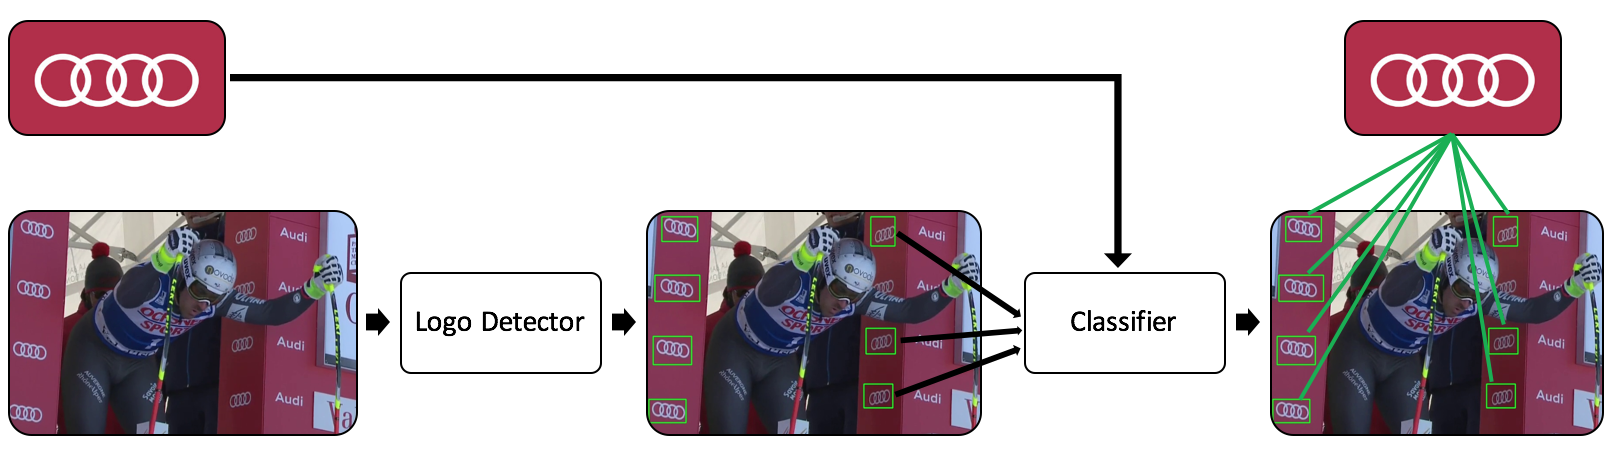
\includegraphics[width=12cm]{images/mt/outline.png}
	\caption{The outline of the proposed system}
	\label{f:outline}
\end{figure}
The challenge of this task is manifold. The first problem is that the logos in these videos are far from being perfectly clear. They can be partially occluded, blurred - if the camera moves fast, perspectively transformed, rotated and can have various coloring, suiting well to the design of the shirt or the arena. In addition, there is a problem with the ambient illumination variation just as for other computer vision tasks.
The second challenge is due to the legal prohibition of copying symbols. This already results in a huge appearance variety, which is further grown by the diversity of logos within a company. This makes the detection of logos very complex. In addition, a lot of companies use wordmarks i.e. a logo only with its name. For a system, not prepared for text recognition, it is a harder task to recognize complete words than only a letter or a simple graphic mark, symbol. These problems make the task of logo retrieval to an open-set recognition problem.
Furthermore, in classification tasks, the objects to be classified have usually a 3D shape in the reality, whereas logos have only a planar surface. It means, that it does not yield additional information, if a logo is photographed from multiple different angles, unlike in case of other objects.
Unfortunately, there are only a few publicly available small datasets with bounding box annotated logos. The majority of the images are adjusted to ensure a good visibility of the logos, unlike on the frames of the sport videos.
Figure \ref{f:challenges} introduces some examples of the challenges.
\begin{figure}
  \centering
  \begin{tabular}{ccccc}
  
\includegraphics[height=15mm]{images/mt/challenge_1_a.png} &   
\includegraphics[width=25mm]{images/mt/challenge_2_a.png}  & 
\includegraphics[width=25mm]{images/mt/challenge_3_a.png} &   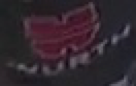
\includegraphics[width=25mm]{images/mt/challenge_4_a.png} & 
\includegraphics[width=25mm]{images/mt/challenge_5_a.png} \\
    
\includegraphics[width=25mm]{images/mt/challenge_1_b.png} &   
\includegraphics[width=25mm]{images/mt/challenge_2_b.png}  & 
\includegraphics[width=25mm]{images/mt/challenge_3_b.png} &   
\includegraphics[width=25mm]{images/mt/challenge_4_b.png}  & 
\includegraphics[width=25mm]{images/mt/challenge_5_b.png} 
    \end{tabular}
    \caption{Examples for challenging logos, where the instances of each column belong to the same class}
    \label{f:challenges}
\end{figure}
To master these challenges, the available solutions and methods improved a lot recently. In the decade before, hand-crafted feature extraction was prevalent in computer vision tasks. It needed an expert to create a system and it yielded often only mediocre results. Deep learning methods for computer vision problems have been dominant since the success of Convolutional Neural Networks in 2012 \cite{NIPS2012_4824}. Compared to earlier systems (e.g. Scale and Translation Invariant Features \cite{Lowe:2004:DIF:993451.996342}, Histogram of Oriented Gradients \cite{Dalal:2005:HOG:1068507.1069007} features), the great improvement of deep learning methods is the capability of learning how to extract features automatically. The enhancements are encouraged by continuous research. The development of deep nets is mainly powered by the annually organized ImageNet classification challenge \cite{ILSVRC15}. Since the aim of this contest is to classify an object, which fills out the majority of an image, the location of the particular object is irrelevant. To be able to classify and recognize objects, which have a much smaller size relative to the size of the whole image, region-based classification can be utilized.
\bigbreak
The rest of this thesis is organized as follows. Chapter \ref{c:relatedwork} reviews the related work of image retrieval, object detection and logo retrieval. In chapter \ref{c:theory} the proposal based object detection with Convolutional Neural Networks will be introduced. Chapter \ref{c:logoretrievalsystem} describes the logo retrieval system. Chapter \ref{c:experiments} presents some experiments to extend the size of the dataset, and evaluates different methods on a standard dataset. Afterwards, chapter \ref{c:evaluation} includes evaluation and comparison of the system with another logo retrieval methods. Finally, the last chapter concludes the work and gives prospects on future work.